\documentclass[conference]{IEEEtran}
\IEEEoverridecommandlockouts

% ---------------------------------------------------------------- packages
\usepackage{cite}
\usepackage{amsmath,amssymb,amsfonts}
\usepackage{graphicx}
\usepackage{textcomp}
\usepackage{xcolor}
\usepackage{booktabs}
\usepackage{multirow}
\usepackage{array}
\usepackage{tabularx}
\usepackage{listings}
\usepackage{pgfplots}
\usepackage{pgfplotstable}
\usepackage[hidelinks]{hyperref}
\pgfplotsset{compat=1.18}
\usepgfplotslibrary{groupplots}
\usetikzlibrary{positioning}

\definecolor{burgundy}{HTML}{8B1E3F}
\definecolor{seriesA}{HTML}{2A78D6}
\definecolor{seriesB}{HTML}{EB6834}
\definecolor{seriesC}{HTML}{1BAF7A}
\definecolor{seriesD}{HTML}{6250D6}
\definecolor{critical}{HTML}{D03B3B}
\definecolor{codebg}{HTML}{F6F6F4}

\lstdefinestyle{py}{
  language=Python, basicstyle=\ttfamily\scriptsize, backgroundcolor=\color{codebg},
  keywordstyle=\color{burgundy}\bfseries, commentstyle=\color{gray}\itshape, stringstyle=\color{seriesA!80!black},
  frame=single, rulecolor=\color{gray!40}, breaklines=true, columns=fullflexible, showstringspaces=false,
  xleftmargin=2pt, xrightmargin=2pt, aboveskip=4pt, belowskip=2pt, captionpos=b, abovecaptionskip=4pt, literate={→}{{$\rightarrow$}}1
}

% Numbers produced by report/generate_report_data.py
% Generated by report/generate_report_data.py -- do not edit by hand
\newcommand{\ParseSeconds}{5.6}
\newcommand{\NLinks}{1{,}214}
\newcommand{\NLines}{19}
\newcommand{\NStations}{482}
\newcommand{\NIntervals}{96}
\newcommand{\NObs}{116{,}544}
\newcommand{\NEligDemand}{116{,}352}
\newcommand{\NEligService}{116{,}352}
\newcommand{\NAmbiguousLinks}{2}
\newcommand{\ZeroObs}{5{,}770}
\newcommand{\ZeroDemand}{163{,}247}
\newcommand{\NExcludedObs}{192}
\newcommand{\PctEligService}{99.8}
\newcommand{\ZeroObsPct}{4.96}
\newcommand{\ZeroDemandPct}{0.41}
\newcommand{\ZeroAdjacentPct}{85}
\newcommand{\NLabelVariants}{19}
\newcommand{\NOrderDiffs}{13}
\newcommand{\ZeroFirstHourPct}{33}
\newcommand{\ZeroLatePct}{22}
\newcommand{\ZeroTopLine}{Elizabeth Line}
\newcommand{\ZeroTopLinePass}{37{,}386}
\newcommand{\NetPeakInterval}{08:15--08:30}
\newcommand{\NetPeakDemand}{1{,}050{,}908}
\newcommand{\NetDailyDemand}{39{,}411{,}202}
\newcommand{\NetDailyTrains}{256{,}422}
\newcommand{\NetPMPeakInterval}{17:45}
\newcommand{\NetPMPeakDemand}{1{,}050{,}013}
\newcommand{\PctPeak}{52.0}
\newcommand{\TopLink}{Farringdon $\rightarrow$ Liverpool Street LU (Elizabeth Line)}
\newcommand{\TopLinkDemand}{193{,}615}
\newcommand{\NOverCap}{226}
\newcommand{\NOverCapLinks}{64}
\newcommand{\NUnderUsed}{51{,}901}
\newcommand{\PctUnderUsed}{61.6}
\newcommand{\MaxLFLine}{LO Weaver}
\newcommand{\MaxLF}{156}
\newcommand{\MaxLFLineOver}{163}
\newcommand{\SecondOverLine}{Elizabeth Line}
\newcommand{\SecondOverCount}{41}
\newcommand{\NLinesWithOver}{7}
\newcommand{\CaseMaxLF}{66}
\newcommand{\WorstOverLink}{Stratford $\rightarrow$ Whitechapel (Elizabeth Line, 08:30)}
\newcommand{\WorstOverLF}{119}
\newcommand{\NetMOneAlloc}{108{,}124}
\newcommand{\NetMOneObserved}{256{,}422}
\newcommand{\NetMOneReductionPct}{57.8}
\newcommand{\NetMOneAllocInclude}{113{,}885}
\newcommand{\NetZeroExtraAlloc}{5{,}761}
\newcommand{\NetMOneSeconds}{8.4}
\newcommand{\NetMOneObs}{110{,}582}
\newcommand{\HighestRatioLine}{LO Liberty}
\newcommand{\HighestRatio}{100}
\newcommand{\LowestRatioLine}{Victoria}
\newcommand{\LowestRatio}{31}
\newcommand{\NoServiceLines}{London Trams}
\newcommand{\CaseLine}{Victoria}
\newcommand{\CaseCap}{986}
\newcommand{\CaseLinks}{30}
\newcommand{\CaseObs}{2{,}880}
\newcommand{\CaseDemand}{2{,}975{,}891}
\newcommand{\CaseObserved}{16{,}228}
\newcommand{\CasePeakFreq}{10}
\newcommand{\CasePeakInterval}{08:30}
\newcommand{\CasePeakLink}{Euston LU $\rightarrow$ Warren Street}
\newcommand{\CasePeakLinkDemand}{5{,}877}
\newcommand{\CaseMOneAlloc}{5{,}049}
\newcommand{\CaseMOneRed}{68.9}
\newcommand{\CaseMOneUtil}{59.7}
\newcommand{\CaseMOneMinTwo}{6{,}046}
\newcommand{\CaseMOneMinFour}{9{,}640}
\newcommand{\CaseMOneMinFourUtil}{31.3}
\newcommand{\CaseMOneExistingShort}{0}
\newcommand{\CaseMTwoSat}{100.000}
\newcommand{\CaseMTwoUnmet}{0}
\newcommand{\CaseMTwoAlloc}{5{,}049}
\newcommand{\CaseMTwoBinding}{0}
\newcommand{\CaseMTwoQSat}{87.53}
\newcommand{\CaseMTwoQBinding}{74}
\newcommand{\CaseMThreeAlloc}{4{,}164}
\newcommand{\CaseMThreeSat}{98.93}
\newcommand{\CaseMThreeE}{5{,}049}
\newcommand{\CaseMTwoInclUnmet}{1{,}779}
\newcommand{\MTwoFullAtBudget}{50}
\newcommand{\MThreeDemandAlloc}{4{,}371}
\newcommand{\MThreeDemandSat}{99.86}
\newcommand{\MThreePatternFiveAlloc}{5{,}049}
\newcommand{\MThreePatternFiveSat}{100.00}
\newcommand{\MThreePatternTwentyAlloc}{16{,}228}
\newcommand{\MThreePatternTwentySat}{100.00}
\newcommand{\MThreeUtilAlloc}{3{,}811}
\newcommand{\MThreeUtilSat}{96.56}
\newcommand{\MThreeEffAlloc}{4{,}164}
\newcommand{\MThreeEffSat}{98.93}
\newcommand{\SensMOneBase}{5{,}049}
\newcommand{\SensMOneTwenty}{5{,}735}
\newcommand{\SensMOneTwentyPct}{13.6}
\newcommand{\SensMOneTen}{5{,}383}
\newcommand{\SensMOneTenPct}{6.6}
\newcommand{\SensMOneRhoSeventy}{5{,}546}
\newcommand{\SensMOneRhoHundred}{4{,}271}
\newcommand{\SensMOneBudgetFeasible}{feasible}
\newcommand{\InfeasStatus}{Infeasible}
\newcommand{\InfeasDiag}{25 observation(s) need more trains than the maximum frequency (10)}
\newcommand{\Rho}{80}


% UI screenshot: uses figures/<file> if present, otherwise prints a placeholder box.
\newcommand{\uishot}[3]{%
\begin{figure*}[!t]\centering
\IfFileExists{figures/#1}{\includegraphics[width=0.9\textwidth,height=0.4\textheight,keepaspectratio]{figures/#1}}{%
\fbox{\parbox[c][0.22\textheight][c]{0.85\textwidth}{\centering\small\textcolor{gray}{Screenshot placeholder:\\ \texttt{figures/\detokenize{#1}}}}}}
\caption{#2}\label{#3}
\end{figure*}}

\newcommand{\Ceff}{C^{\mathrm{eff}}}
% Generated table rows; the TeX primitive input is expandable, so \bottomrule may follow it.
\makeatletter\newcommand{\tabinput}[1]{\@@input #1 }\makeatother

\begin{document}

\title{Data-Driven Urban Metro Train Frequency and Capacity Optimization Using Transport for London NUMBAT Data}

\author{
\IEEEauthorblockN{Arunoday A K}
\IEEEauthorblockA{\textit{School of AI}\\
\textit{Amrita Vishwa Vidyapeetham}\\
Coimbatore, India\\
CB.SC.U4AIE23106}
\and
\IEEEauthorblockN{Achutharaj R}
\IEEEauthorblockA{\textit{School of AI}\\
\textit{Amrita Vishwa Vidyapeetham}\\
Coimbatore, India\\
CB.SC.U4AIE23108}
\and
\IEEEauthorblockN{D Lokesh}
\IEEEauthorblockA{\textit{School of AI}\\
\textit{Amrita Vishwa Vidyapeetham}\\
Coimbatore, India\\
CB.SC.U4AIE23123}
\and
\IEEEauthorblockN{Abhay Rohit M}
\IEEEauthorblockA{\textit{School of AI}\\
\textit{Amrita Vishwa Vidyapeetham}\\
Coimbatore, India\\
CB.SC.U4AIE23173}
\and
\IEEEauthorblockN{Dr. Shyam A V\IEEEauthorrefmark{1}}
\IEEEauthorblockA{\textit{Assistant Professor, School of AI}\\
\textit{Amrita Vishwa Vidyapeetham}\\
Coimbatore, India\\
\IEEEauthorrefmark{1}Faculty Mentor}
\thanks{Course project for 23MNG336 Operations Research.}
}

\maketitle

% ================================================================ ABSTRACT
\begin{abstract}
Urban metro demand varies strongly across the day and across the network, while train frequencies are fixed by
timetables. This paper presents a data-driven decision-support system that uses Transport for London's NUMBAT
open data to (i)~profile and validate link-level passenger loads and scheduled train frequencies, and (ii)~solve three
Operations Research models: an integer program for the minimum train frequency that carries observed demand, a
two-stage mixed-integer program that allocates a limited link-service budget to maximise demand served, and a
weighted goal program that balances operating effort, demand satisfaction, adherence to the existing service pattern
and a target capacity utilisation. The NUMBAT 2025 workbook yields \NObs{} link--interval observations
(\NLinks{} links, \NLines{} lines, \NIntervals{} quarter-hours). A consistency check requested at the first review found
\ZeroObs{} observations (\ZeroDemandPct\% of demand) where passengers are reported on a link with zero scheduled trains;
these are flagged and handled by an explicit, user-selectable policy. With published rolling-stock capacities and an
\Rho\% utilisation target, the minimum-frequency model needs \NetMOneReductionPct\% fewer link-train allocations than
the timetable network-wide, showing that observed frequencies are set by headway standards rather than by volume alone.
Scenario analysis quantifies the effect of 10--20\% demand growth, reduced service budgets and alternative
utilisation targets. The models are implemented in Pyomo with the HiGHS solver and delivered through an interactive
Streamlit dashboard.
\end{abstract}

\begin{IEEEkeywords}
train frequency setting, integer programming, goal programming, capacity allocation, public transport, NUMBAT,
Transport for London, Pyomo, HiGHS, decision support
\end{IEEEkeywords}

% ================================================================ I. INTRODUCTION
\section{Introduction}
Metro systems carry large and highly variable passenger volumes. Demand peaks sharply in the morning and evening,
differs between lines and between consecutive segments of the same line, and falls to very low levels late at night.
Train frequency, on the other hand, is planned in advance and constrained by rolling stock, crews and signalling.
When the two are misaligned, passengers experience overcrowding on busy segments while trains on quiet segments
run with spare capacity~\cite{ceder2016,ibarra2015}.

\textbf{Why this matters.} From a passenger perspective, matching capacity to demand reduces crowding and keeps
service levels consistent. From an operator perspective, it identifies demand--service mismatches and avoids
unnecessary service in low-demand periods. For decision makers, it replaces fixed rules of thumb with quantitative,
reproducible recommendations whose sensitivity to demand growth and resource limits can be tested before any change
is made.

Transport for London (TfL) publishes the NUMBAT dataset~\cite{tfl_numbat}, which reports, for every link between
consecutive stations and every 15-minute interval of a typical day, both the passenger load and the number of
scheduled trains. Having demand and supply at the same resolution makes NUMBAT well suited to frequency and
capacity optimisation.

\textbf{Contributions.} This work
\begin{enumerate}
\item builds a schema-detecting parser and validation pipeline that turns the wide-format NUMBAT workbook into a
      clean, key-matched link--interval table with a transparent data-quality report;
\item formulates and solves three distinct Operations Research models (integer programming, mixed-integer
      allocation and weighted goal programming) on the real data, with post-solve verification of every solution;
\item explicitly diagnoses and handles observations where demand is reported without any scheduled train, the issue
      raised at the first review (Section~\ref{sec:review});
\item performs scenario and sensitivity analysis on demand, budget and utilisation targets; and
\item delivers everything through an interactive dashboard that a non-programmer can use with an unmodified
      workbook downloaded from TfL.
\end{enumerate}

The remainder of the paper is organised as follows. Section~\ref{sec:related} reviews related work,
Section~\ref{sec:data} describes the dataset and Section~\ref{sec:questions} the research questions.
Section~\ref{sec:method} presents the methodology and models, Section~\ref{sec:impl} the implementation and user
interface, Section~\ref{sec:results} the results and Section~\ref{sec:review} the response to the first-review
feedback. Section~\ref{sec:discussion} discusses limitations and Section~\ref{sec:conclusion} concludes.

% ================================================================ II. RELATED WORK
\section{Related Work}\label{sec:related}
Frequency setting is a classical stage of transit planning, following network design and preceding timetabling,
vehicle scheduling and crew scheduling~\cite{guihaire2008,desaulniers2007,ibarra2015}. The simplest and most widely
used rule is the \emph{maximum-load-point} method, which sets the frequency on a route to the peak load divided by
the desired occupancy per vehicle~\cite{ceder2016}. Ceder~\cite{ceder2016} refines this with load-profile methods that
use the load on every segment rather than only at the peak point, which is the link-level view adopted here.
Furth and Wilson~\cite{furth1981} formulated frequency allocation across routes as a resource-constrained
optimisation that maximises net social benefit subject to a fleet budget, the conceptual basis of our Model~2.

When several conflicting objectives must be balanced, goal programming~\cite{charnes1961,tamiz1998,jones2010} is a
natural tool: each objective becomes a goal with a target, and weighted deviations from the targets are minimised.
Normalisation of the deviations is essential when goals are measured in different units~\cite{tamiz1998,jones2010}.

Open-source algebraic modelling languages such as Pyomo~\cite{hart2011,bynum2021} and high-performance open solvers
such as HiGHS~\cite{huangfu2018} make it practical to embed these models in interactive decision-support tools. Our
work combines these elements with a publicly available, high-resolution demand dataset and places particular emphasis
on data validation, which is often assumed rather than demonstrated in applied studies.

% ================================================================ III. DATASET
\section{Dataset}\label{sec:data}
\subsection{Source and coverage}
NUMBAT is published by TfL Public Transport Service Planning at \url{https://crowding.data.tfl.gov.uk/}~\cite{tfl_numbat}.
It is produced from smartcard ticketing data and gateline entry/exit counts: each journey's route is estimated and
assigned to trains and stations. The data represent a \emph{typical} autumn day (here the 2025 Tuesday--Thursday
average, file \texttt{NBT25TWT\_Outputs.xlsx}) from 05:00 to 04:59, assume a full timetabled service, and cover the
London Underground, London Overground, Docklands Light Railway (DLR), Elizabeth line and London Trams.

\subsection{Workbook structure}
The workbook contains nine worksheets (Table~\ref{tab:sheets}). Each data sheet is in \emph{wide} format: two title
rows (hour and quarter-hour indices), a header row with the field names, then one row per link or station with a
daily total, six time-of-day totals and 96 quarter-hour columns labelled \texttt{0500-0515} to \texttt{0445-0500}.

\begin{table}[!t]
\caption{NUMBAT worksheets and their use in this work}\label{tab:sheets}
\centering\footnotesize
\begin{tabularx}{\columnwidth}{@{}l r X@{}}
\toprule
Sheet & Rows & Content and use \\
\midrule
\texttt{Link\_Loads} & 1{,}214 & Passengers on each link per 15 min. \textbf{Demand $D_i$.} \\
\texttt{Link\_Frequencies} & 1{,}214 & Trains on each link per 15 min (from the timetable). \textbf{Observed supply $f_i$.} \\
\texttt{Line\_Boarders} & 21 & Boardings per line. Not used for optimisation. \\
\texttt{Station\_*} (5 sheets) & 471--5{,}627 & Entries, exits, boarders, alighters, flows. Not substitutes for link loads. \\
\texttt{\_Cover} & -- & Method and data-confidence notes, shown in the app. \\
\bottomrule
\end{tabularx}
\end{table}

\subsection{Variables used}
A \emph{link} is a directed segment between consecutive stations on one line (e.g.\ Victoria line southbound,
Green Park $\rightarrow$ Victoria), identified by a unique code such as \texttt{GPKu\_VIC\_SB>VICu\_VIC\_SB@VIC},
with line, direction, sequence order, NLC/ASC station codes and station names. For link $\ell$ and interval $t$,
the \emph{link load} is the number of passengers traversing the link during the interval, and the \emph{link
frequency} is the number of trains traversing it during the same interval. Frequencies are \emph{trains per
15 minutes}, not trains per hour. Because a passenger is counted on every link they ride, summing link loads gives
passenger-link trips, not unique journeys.

\subsection{Summary statistics}
After preprocessing (Section~\ref{sec:prep}) the dataset contains \NLinks{} links on \NLines{} lines between
\NStations{} stations, giving \NObs{} link--interval observations, of which \NEligService{} (\PctEligService\%) have
validated demand and frequency. Across the network the day totals \NetDailyDemand{} passenger-link trips and
\NetDailyTrains{} link-train allocations. The AM and PM peak periods together account for \PctPeak\% of daily demand.

% ================================================================ IV. QUESTIONS
\section{Research Questions}\label{sec:questions}
\begin{enumerate}
\item[\textbf{Q1}] \textbf{Demand:} what are the temporal and spatial patterns of passenger demand across the network?
\item[\textbf{Q2}] \textbf{Service:} how does the existing train frequency correspond to passenger demand?
\item[\textbf{Q3}] \textbf{Frequency optimisation:} what train frequency is required to satisfy demand under capacity constraints? (Model~1)
\item[\textbf{Q4}] \textbf{Capacity allocation:} given limited service capacity, how should trains be allocated across segments and time periods? (Model~2)
\item[\textbf{Q5}] \textbf{Multi-objective planning:} how can frequency be planned while balancing operating effort, crowding and service quality? (Model~3)
\item[\textbf{Q6}] \textbf{Sensitivity:} how does the optimal solution change when demand, capacity targets or resources change?
\end{enumerate}

% ================================================================ V. METHODOLOGY
\section{Methodology}\label{sec:method}
Fig.~\ref{fig:pipeline} summarises the pipeline. The uploaded workbook is the only source of operational
observations; every assumption not contained in it (capacity per train, utilisation target, frequency bounds and
budget) is an explicit user input.

\begin{figure}[!t]\centering
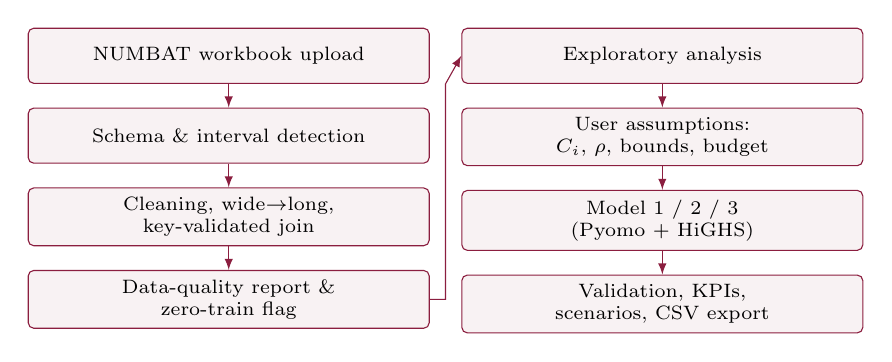
\begin{tikzpicture}[node distance=3mm, every node/.style={font=\scriptsize, align=center},
  box/.style={draw=burgundy, rounded corners=2pt, fill=burgundy!6, minimum width=0.42\columnwidth, minimum height=7mm},
  arr/.style={-latex, burgundy}]
\node[box] (a) {NUMBAT workbook upload};
\node[box, below=of a] (b) {Schema \& interval detection};
\node[box, below=of b] (c) {Cleaning, wide$\rightarrow$long,\\ key-validated join};
\node[box, below=of c] (d) {Data-quality report \&\\ zero-train flag};
\node[box, right=4mm of a] (e) {Exploratory analysis};
\node[box, below=of e] (f) {User assumptions:\\ $C_i$, $\rho$, bounds, budget};
\node[box, below=of f] (g) {Model 1 / 2 / 3\\ (Pyomo + HiGHS)};
\node[box, below=of g] (h) {Validation, KPIs,\\ scenarios, CSV export};
\draw[arr] (a)--(b); \draw[arr] (b)--(c); \draw[arr] (c)--(d);
\draw[arr] (d.east) -| ([xshift=-2mm]e.south west) -- (e.west);
\draw[arr] (e)--(f); \draw[arr] (f)--(g); \draw[arr] (g)--(h);
\end{tikzpicture}
\caption{Processing and optimisation pipeline implemented in the dashboard.}\label{fig:pipeline}
\end{figure}

\subsection{Data parsing}\label{sec:parse}
NUMBAT downloads differ between years and day types, so nothing is read from fixed rows or columns. The parser
(i)~finds the link sheets by name or by their title cell; (ii)~selects as header row the row that matches the most
known field names (with aliases such as \emph{Dir}/\emph{Direction}); and (iii)~recognises interval columns by the
pattern \texttt{HHMM-HHMM}, accepting only 15-minute spans. Intervals are ordered by
$\big((\text{start} - 300) \bmod 1440\big)/15$, so the operating day runs from 05:00 across midnight to 04:59.
Ambiguous header matches are reported rather than resolved silently.

\subsection{Preprocessing and validation}\label{sec:prep}
The two link sheets are cleaned and reshaped from wide to long format (one row per link and interval), then joined.
The rules are:
\begin{itemize}
\item \textbf{Join key.} The first candidate key that exists and is unique in both sheets is used: the link code, then
  line\,+\,direction\,+\,NLC codes, then line\,+\,direction\,+\,station names. The join is on key and interval, never
  on row position. For the 2025 workbook the link code is unique in both sheets.
\item \textbf{Missing is not zero.} Empty, non-numeric and negative cells are flagged and excluded; they are never
  replaced by zero. Genuine zeros are kept.
\item \textbf{Duplicates.} Exact duplicate rows are dropped once; records that share a key with different values are
  \emph{ambiguous} and excluded, never averaged.
\item \textbf{Cross-sheet consistency.} For every matched link the descriptive fields of the two sheets are compared.
  \NLabelVariants{} station labels differ only by a branch qualifier (e.g.\ ``Kennington (Bank)'' vs.\ ``Kennington'')
  and \NOrderDiffs{} links differ only in sequence number; these are reported and kept. \NAmbiguousLinks{} links have
  genuinely conflicting identities (one link's destination is ``Liverpool Street'' in one sheet and ``Hackney Downs''
  in the other; another has a different NLC) and are excluded (\NExcludedObs{} observations).
\item \textbf{Totals.} The daily \emph{Total} column is checked against the sum of the 96 interval values (consistent
  for every link) but is never used as interval demand.
\end{itemize}

\subsection{Demand reported with zero scheduled trains}\label{sec:zero}
A physically consistent observation cannot have passengers on a link in an interval with no train. The dataset
contains \ZeroObs{} such link--intervals (\ZeroObsPct\% of matched observations), carrying \ZeroDemand{} passengers
(\ZeroDemandPct\% of demand). Fig.~\ref{fig:zero} shows that they concentrate at the start and end of the traffic day:
\ZeroFirstHourPct\% of this demand falls between 05:00 and 06:00 and \ZeroLatePct\% after midnight. For
\ZeroAdjacentPct\% of the demand, the same link has trains in the adjacent interval. This indicates a period-boundary
effect: NUMBAT's assigned loads and the timetable assign a train run to slightly different quarter-hours, and the
averaging over several days spreads small loads into neighbouring periods.

Every such observation is flagged (\texttt{zero\_train\_demand}) and reported by line and interval in the Data Quality
tab. Because the right treatment is a modelling decision, it is exposed as a policy:
\begin{itemize}
\item \textbf{Exclude (default):} the observations are removed from optimisation and the removed demand is disclosed
  with every result;
\item \textbf{Include:} the demand is kept, so models may add service where the timetable has none.
\end{itemize}
Section~\ref{sec:results} compares both policies.

\begin{figure}[!t]\centering
\begin{tikzpicture}
\begin{axis}[width=0.95\columnwidth, height=4.2cm, ybar, bar width=0.6pt, ymin=0,
  xlabel={Interval of the operating day (0 = 05:00)}, ylabel={Passengers}, xmin=-1, xmax=96,
  xtick={0,12,28,52,76,95}, xticklabels={05:00,08:00,12:00,18:00,00:00,04:45},
  ylabel style={font=\scriptsize}, xlabel style={font=\scriptsize}, tick label style={font=\scriptsize},
  scaled y ticks=false, yticklabel style={/pgf/number format/fixed}]
\addplot[fill=critical, draw=critical] table[x=interval_order, y=demand, col sep=comma]{data/zero_train_by_interval.csv};
\end{axis}
\end{tikzpicture}
\caption{Passengers reported on link--intervals that have zero scheduled trains, by interval (all lines).}\label{fig:zero}
\end{figure}

\subsection{User-supplied parameters}\label{sec:params}
\textbf{Capacity per train $C_i$.} NUMBAT does not contain vehicle capacity. Default values per line were taken from
TfL rolling-stock data sheets~\cite{tfl_rs4,tfl_345,tfl_378} and, where no TfL sheet was found, from secondary
sources~\cite{wiki_710,wiki_dlr,wiki_tram} (Table~\ref{tab:capacity}). For the Underground they are seats plus standing
room at 5 passengers/m$^2$, which TfL calls the ``maximum observed standing capacity''. All values can be edited in the
dashboard, or replaced by one uniform value, which is then disclosed with every result.

\begin{table}[!t]
\caption{Default capacity per train (editable in the dashboard)}\label{tab:capacity}
\centering\scriptsize
\setlength{\tabcolsep}{4pt}
\begin{tabular}{@{}l l r c@{}}
\toprule
Line & Stock (cars) & $C$ & Source \\
\midrule
Bakerloo & 1972 (7) & 851 & \cite{tfl_rs4} \\
Central & 1992 (8) & 1{,}047 & \cite{tfl_rs4} \\
District, H\&C, Circle & S7 (7) & 1{,}045 & \cite{tfl_rs4} \\
Jubilee & 1996 (7) & 964 & \cite{tfl_rs4} \\
Metropolitan & S8 (8) & 1{,}176 & \cite{tfl_rs4} \\
Northern & 1995 (6) & 752 & \cite{tfl_rs4} \\
Piccadilly & 1973 (6) & 798 & \cite{tfl_rs4} \\
Victoria & 2009 (8) & 986 & \cite{tfl_rs4} \\
Waterloo \& City & 1992 (4) & 506 & \cite{tfl_rs4} \\
Elizabeth line & Class 345 (9) & 1{,}497 & \cite{tfl_345} \\
LO Mildmay, Windrush & Class 378 (5) & 840 & \cite{tfl_378} \\
LO Liberty, Weaver & Class 710 (4) & 678 & \cite{wiki_710} \\
LO Suffragette, Lioness & Class 710 (4) & 678 & \cite{wiki_710} \\
DLR & B07/B2K (3) & 688 & \cite{wiki_dlr} \\
London Trams & Variobahn & 206 & \cite{wiki_tram} \\
\bottomrule
\end{tabular}
\end{table}

\textbf{Target utilisation $\rho$.} The usable capacity is $\Ceff_i = \rho\,C_i$ with $0 < \rho \le 1$, a planning buffer
below rated capacity. The default is $\rho = \Rho\%$, a modelling choice and not a TfL value.

\textbf{Frequency bounds.} Optional minimum $l$ and maximum $u$ trains per link per 15 minutes, with $l \le u$
enforced. The minimum can be applied only where the link is observed in service, so that overnight closures are not
forced open.

\textbf{Link-service allocation budget.} The workbook gives trains per link, not the number of physical trains, and one
train traverses many consecutive links. We therefore define a \emph{link-service allocation budget}
\begin{equation}
F_t = \Big\lfloor \beta \sum_{i \in t} f_i \Big\rfloor,
\end{equation}
where $\beta$ is a user-chosen fraction of the observed allocations in interval $t$. $F_t$ is a modelling resource, not
a fleet count.

\subsection{Notation}
Index $i$ denotes one (link, interval) observation and $t$ an interval; $i \in t$ means observation $i$ belongs to
interval $t$. $D_i$ is observed demand, $f_i$ observed trains, $C_i$ rated capacity and $\Ceff_i = \rho C_i$.
Decision variables are $x_i \in \mathbb{Z}_{\ge 0}$ (train allocations) and $y_i \ge 0$ (passengers served).

\subsection{Model 1: minimum train frequency (integer programming)}
\begin{align}
\min\ & \sum_i x_i \label{eq:m1obj}\\
\text{s.t.}\ & \Ceff_i\, x_i \ge D_i && \forall i \label{eq:m1cap}\\
& l_i \le x_i \le u_i,\ \ x_i \in \mathbb{Z}_{\ge 0} && \forall i \\
& \textstyle\sum_{i \in t} x_i \le F_t && \forall t \quad \text{(optional)} \label{eq:m1bud}
\end{align}
Without~\eqref{eq:m1bud} the problem separates and the optimum is $x_i^* = \max(l_i, \lceil D_i / \Ceff_i \rceil)$; the
solver output is tested against this closed form. If a maximum frequency or the budget cannot cover demand, the model
is reported as infeasible and the conflicting links or intervals are listed. Constraints are never relaxed silently.

\subsection{Model 2: capacity-constrained service allocation (MILP)}
\begin{align}
\max\ & \sum_i y_i \\
\text{s.t.}\ & 0 \le y_i \le D_i && \forall i \\
& y_i \le \Ceff_i\, x_i && \forall i \\
& \textstyle\sum_{i \in t} x_i \le F_t && \forall t \\
& l_i \le x_i \le \bar u_i,\ \ x_i \in \mathbb{Z}_{\ge 0} && \forall i
\end{align}
with $\bar u_i = \min\!\big(u_i, \max(l_i, \lceil D_i/\Ceff_i\rceil)\big)$. The bound $\lceil D_i/\Ceff_i\rceil$ is a
valid technical bound: more trains cannot serve more passengers. The
objective does not penalise allocations, so several optima may contain trains that serve nobody. A lexicographic
second stage~\cite{williams2013} therefore minimises $\sum_i x_i$ subject to $\sum_i y_i \ge (1-10^{-8})\,Y^*$, where
$Y^*$ is the stage-1 optimum. An interval is reported as \emph{binding} when $\sum_{i\in t}x_i = F_t$ and demand in that interval is left unmet, i.e.\ the budget actually limits service.

\subsection{Model 3: weighted goal programming}
Model~3 uses rated capacity as the hard limit, $y_i \le \min(D_i, C_i x_i)$, and treats the utilisation target as a
soft goal. Four goals are expressed with non-negative deviation variables $p, n$:
\begin{align}
\text{G1 (effort):}\ & \textstyle\sum_i x_i - E = p_1 - n_1 \\
\text{G2 (demand):}\ & \text{unmet} = \textstyle\sum_i (D_i - y_i) \\
\text{G3 (pattern):}\ & x_i - f_i = p_{3i} - n_{3i} && \forall i \\
\text{G4 (utilisation):}\ & D_i - \rho C_i x_i = p_{4i} - n_{4i} && \forall i
\end{align}
where $E = \sum_i \max(l_i, \lceil D_i/\Ceff_i\rceil)$ is the least effort that carries all demand at the target
utilisation. With percentage normalisation~\cite{tamiz1998,jones2010}, each deviation is divided by its goal target:
\begin{equation}
\begin{split}
\min\ & w_1\frac{p_1}{E} + w_2\frac{\text{unmet}}{\sum_i D_i} \\
& + w_3\frac{\sum_i(p_{3i}+n_{3i})}{\sum_i f_i} + w_4\frac{\sum_i(p_{4i}+n_{4i})}{\sum_i D_i}.
\end{split}
\end{equation}
The weights $w_k$ start equal and are user settings. G2 and G4 are related but distinct: $p_{4i}$ counts load above
the target $\rho C_i$, while unmet demand arises only above the rated capacity $C_i$. NUMBAT does not observe crowding
directly, so G4 is derived from link loads and the capacity assumption.

Two numerical safeguards are used. First, a weight of $10^{-3}$ on every goal breaks ties when a user sets a weight
to zero, so solutions stay Pareto-efficient. Second, the objective is multiplied by a constant
$\max(E, \sum f_i, \sum D_i)$. Without this scaling, cost coefficients near $10^{-8}$ were treated as zero by the HiGHS
presolve, which then returned a meaningless ``optimal'' plan; the post-solve checks below detected this.

\subsection{Scenario and sensitivity analysis}
Each model can be re-solved under: (A)~baseline; (B)~$D_i' = 1.10D_i$; (C)~$D_i' = 1.20D_i$; (D)~the allocation budget
reduced by a chosen percentage; and (E)~alternative utilisation targets $\rho$. Scenario D reduces the modelled
budget, not TfL's physical fleet. Infeasible scenarios are reported as infeasible.

\subsection{Solution verification}
HiGHS~\cite{huangfu2018} is called through Pyomo~\cite{bynum2021} with a time limit and a relative MIP gap of
$10^{-4}$. A result is shown only if a solution exists. It is labelled ``optimal'' only if HiGHS proves optimality and
the primal and dual bounds agree. Independent checks then verify integrality, bounds, $y_i \le D_i$,
$y_i \le$ capacity $\times\, x_i$, demand coverage (Model~1) and the budget in every interval. A failed check suppresses
the result.

% ================================================================ VI. IMPLEMENTATION
\section{Implementation and User Interface}\label{sec:impl}
\subsection{Architecture}
The system is written in Python with a deliberately small codebase (Table~\ref{tab:modules}): pandas and NumPy for data
processing~\cite{mckinney2010}, Pyomo with HiGHS for optimisation, Plotly for charts, NetworkX~\cite{hagberg2008} for the
network view, Streamlit~\cite{streamlit} for the interface and pytest for 24 automated tests.

\begin{table}[!t]
\caption{Code modules}\label{tab:modules}
\centering\footnotesize
\begin{tabularx}{\columnwidth}{@{}l X@{}}
\toprule
Module & Responsibility \\
\midrule
\texttt{data\_loader.py} & Sheet, header-row, field-alias and interval detection; cover notes \\
\texttt{preprocessing.py} & Cleaning, reshaping, key-validated join, quality metrics, zero-train flag, readiness \\
\texttt{optimization.py} & Models 1--3, result tables, KPIs, post-solve validation \\
\texttt{analysis.py} & Descriptive summaries, interpretation text, scenario runner \\
\texttt{visualization.py} & Plotly charts and schematic network \\
\texttt{app.py} & Streamlit dashboard (five tabs) \\
\texttt{tests/} & 24 unit and integration tests \\
\bottomrule
\end{tabularx}
\end{table}

\subsection{Code excerpts}
Listing~\ref{lst:zero} shows how the zero-train observations are flagged, and Listing~\ref{lst:m2} the core of
Model~2, including the second stage.

\begin{lstlisting}[style=py, float=tp, caption={Flagging zero-train demand (\texttt{preprocessing.py}).}, label={lst:zero}]
merged["zero_train_demand"] = (merged["eligible_service"]
    & (merged["frequency"] == 0) & (merged["demand"] > 0))
grp = merged.groupby("link_key")
adjacent = pd.Series(False, index=merged.index)
for step in (1, -1):   # trains on the same link in the next/previous interval?
    nxt = grp["interval_order"].shift(-step) == merged["interval_order"] + step
    adjacent |= nxt & (grp["frequency"].shift(-step) > 0)
merged["zero_train_adjacent_service"] = merged["zero_train_demand"] & adjacent
\end{lstlisting}

\begin{lstlisting}[style=py, float=tp, caption={Two-stage Model 2 in Pyomo (\texttt{optimization.py}).}, label={lst:m2}]
tech_ub = np.ceil(D / Ce - 1e-9)        # more trains cannot serve more
m = _base_model(w, _x_bounds(w, tech_ub), budgets)  # x_i, budget rows
m.y = pyo.Var(m.I, within=pyo.NonNegativeReals,
              bounds=lambda _, i: (0, D[i]))
m.served_cap = pyo.Constraint(m.I,
              rule=lambda m, i: m.y[i] <= Ce[i] * m.x[i])
m.obj = pyo.Objective(expr=sum(m.y[i] for i in m.I), sense=pyo.maximize)
sol1 = _solve(m, s)                     # stage 1: max served demand
best = sum(_values(m.y, len(w)))
m.obj.deactivate()                      # stage 2: same service, fewer trains
m.keep_served = pyo.Constraint(
    expr=sum(m.y[i] for i in m.I) >= best - max(1e-8 * best, 1e-4))
m.obj2 = pyo.Objective(expr=sum(m.x[i] for i in m.I), sense=pyo.minimize)
sol2 = _solve(m, s)
\end{lstlisting}

\subsection{Dashboard}
A user uploads the unmodified workbook. The sidebar holds the scope (lines, directions, time window), capacity
assumptions, service constraints and the zero-train policy. Five tabs follow the analysis workflow:
\textbf{Overview} (readiness per model, scope KPIs, demand and service profile, cover-sheet notes; Fig.~\ref{fig:ui1}),
\textbf{Data Quality} (profiling, preprocessing log, exclusions, zero-train analysis and the processed-data download;
Fig.~\ref{fig:ui2}), \textbf{Explore Data} (top links and lines, peak vs.\ off-peak, demand heatmap, demand vs.\ service,
mismatch tables and a schematic network; Fig.~\ref{fig:ui3}), \textbf{Optimization} (model choice, formulation,
parameters, the \emph{Optimize} button, KPIs, generated interpretation, before/after charts, goal deviations,
validation checks and CSV download; Fig.~\ref{fig:ui4}) and \textbf{Sensitivity Analysis} (scenario selection,
comparison table, chart and CSV; Fig.~\ref{fig:ui5}). Every result is displayed together with the dataset, scope and
assumptions that produced it. Results are invalidated when a different workbook is uploaded.

\uishot{ui_overview.png}{Overview tab: sidebar inputs, readiness of each model, scope KPIs and the demand/service profile.}{fig:ui1}
\uishot{ui_data_quality.png}{Data Quality tab: sheet profile, join coverage, preprocessing log and the zero-train analysis.}{fig:ui2}
\uishot{ui_explore.png}{Explore Data tab: demand heatmap and schematic network topology (not a geographic map).}{fig:ui3}
\uishot{ui_optimization.png}{Optimization tab: assumptions, solver status, KPIs, interpretation and before/after comparison.}{fig:ui4}
\uishot{ui_sensitivity.png}{Sensitivity Analysis tab: scenario comparison table and chart.}{fig:ui5}

% ================================================================ VII. RESULTS
\section{Results}\label{sec:results}
Unless stated otherwise, results use the default capacities (Table~\ref{tab:capacity}), $\rho = \Rho\%$, no minimum or
maximum frequency, a budget equal to the observed allocations ($\beta = 1$) and the \emph{exclude} zero-train policy.
All numbers are produced by \texttt{report/generate\_report\_data.py} from the same code as the dashboard.

\subsection{Q1: demand patterns}
Fig.~\ref{fig:profile} shows the network demand and service profiles. Demand peaks at \NetPeakInterval{}
(\NetPeakDemand{} passenger-link trips in one quarter-hour), with a second, broader evening peak around
\NetPMPeakInterval{} (\NetPMPeakDemand). Table~\ref{tab:lines} breaks demand down by line. The busiest single link is
\TopLink{} with \TopLinkDemand{} passengers per day (Table~\ref{tab:toplinks}).

\begin{figure}[!t]\centering
\begin{tikzpicture}
\begin{groupplot}[group style={group size=1 by 2, vertical sep=6mm, xticklabels at=edge bottom},
  width=\columnwidth, height=3.6cm, xmin=5, xmax=29, xtick={5,8,11,14,17,20,23,26,29},
  xticklabels={05,08,11,14,17,20,23,02,05}, tick label style={font=\scriptsize},
  ylabel style={font=\scriptsize}, scaled y ticks=false, yticklabel style={/pgf/number format/fixed}, ymin=0]
\nextgroupplot[ylabel={Passengers (000s)}]
\addplot[seriesA, thick, const plot] table[x=hour, y expr=\thisrow{demand}/1000, col sep=comma]{data/network_profile.csv};
\nextgroupplot[ylabel={Link-train allocations}, xlabel={Time of day}, xlabel style={font=\scriptsize}]
\addplot[seriesB, thick, const plot] table[x=hour, y=frequency, col sep=comma]{data/network_profile.csv};
\end{groupplot}
\end{tikzpicture}
\caption{Network-wide link demand (top) and scheduled link-train allocations (bottom) per 15 minutes, 05:00--04:59.}\label{fig:profile}
\end{figure}

\begin{table}[!t]
\caption{Daily demand (thousand passenger-link trips), observed link-train allocations, passengers per allocation and
observed load factor $D_i/(C_i f_i)$ in \% of rated capacity, by line}\label{tab:lines}
\centering\scriptsize
\setlength{\tabcolsep}{2.5pt}
\resizebox{\columnwidth}{!}{%
\begin{tabular}{@{}l r r r r r r@{}}
\toprule
Line & Links & Demand & Alloc. & Pass./alloc. & Mean LF & Max LF \\
\midrule
\tabinput{data/tab_lines.tex}
\bottomrule
\end{tabular}}
\end{table}

\begin{table*}[!t]
\caption{Ten highest-demand links (passengers per day and in the busiest quarter-hour)}\label{tab:toplinks}
\centering\footnotesize
\begin{tabular}{@{}r l l r r@{}}
\toprule
\# & Link & Line & Daily & Peak 15 min \\
\midrule
\tabinput{data/tab_top_links.tex}
\bottomrule
\end{tabular}
\end{table*}

\subsection{Q2: how service corresponds to demand}
Service follows the shape of demand (Fig.~\ref{fig:profile}) but is much flatter: trains run at near-peak
frequencies through the inter-peak period, when demand is far lower. Comparing demand with the observed effective
capacity $f_i\,\rho\,C_i$ (only where $f_i > 0$; zero-train records are treated in Section~\ref{sec:zero}),
\NOverCap{} link--intervals on \NOverCapLinks{} links of \NLinesWithOver{} lines carry more than \Rho\% of rated
capacity. They are concentrated on the \MaxLFLine{} (\MaxLFLineOver) and \SecondOverLine{} (\SecondOverCount) lines.
The highest load factor, \MaxLF\%, occurs on the \MaxLFLine{} line. That value is partly an artefact of the
conservative 4-car capacity assumed in Table~\ref{tab:capacity}, since some peak services there run as 8-car pairs.
The largest excess in passengers is on \WorstOverLink{} at \WorstOverLF\% of the Class 345 full-load capacity.
At the other extreme, \NUnderUsed{} link--intervals with trains (\PctUnderUsed\%) run below 15\% of rated capacity.
Mean load factors (Table~\ref{tab:lines}) are low because they average over the whole day, while the maxima show
where peak crowding occurs. The \NoServiceLines{} rows of this workbook contain zero demand and zero frequency in
every interval, so they are excluded from the line comparisons.

\subsection{Q3: minimum frequency (Model 1)}
Network-wide, Model~1 solves all \NetMOneObs{} eligible observations in \NetMOneSeconds{}\,s and needs \NetMOneAlloc{}
link-train allocations against \NetMOneObserved{} observed, i.e.\ \NetMOneReductionPct\% fewer.
Table~\ref{tab:m1lines} shows the ratio per line. The ratio is highest on the \HighestRatioLine{} line (\HighestRatio\%)
and lowest on the \LowestRatioLine{} line (\LowestRatio\%). The reduction does not mean that TfL over-supplies service.
Model~1 sizes service to passenger volume only, while real timetables also provide short waiting times and regular
headways. This is shown by the minimum-frequency experiments in the case study below.

\begin{table}[!t]
\caption{Model 1 network-wide: observed vs.\ minimum required link-train allocations per day, and peak allocations per 15 min on any link}\label{tab:m1lines}
\centering\scriptsize
\setlength{\tabcolsep}{3pt}
\begin{tabular}{@{}l r r r r r@{}}
\toprule
Line & Observed & Required & Ratio & Peak obs. & Peak req. \\
\midrule
\tabinput{data/tab_model1_lines.tex}
\bottomrule
\end{tabular}
\end{table}

\textbf{Effect of the zero-train policy.} With the \emph{include} policy, Model~1 needs \NetMOneAllocInclude{}
allocations, \NetZeroExtraAlloc{} more than under \emph{exclude}. These extra trains would run in quarter-hours where
the timetable has none, to carry only \ZeroDemandPct\% of demand. This confirms that treating the inconsistent records
uncritically would distort the recommendations, which was the concern raised at the review.

\subsection{Case study: the \CaseLine{} line}
The \CaseLine{} line has \CaseLinks{} links (two directions) and \CaseObs{} eligible observations, carrying
\CaseDemand{} passenger-link trips on \CaseObserved{} observed allocations, with up to \CasePeakFreq{} trains per
link per 15 minutes. Its busiest observation is \CasePeakLink{} at \CasePeakInterval{} (\CasePeakLinkDemand{}
passengers in 15 minutes). We use $C = \CaseCap$ (2009 stock). Table~\ref{tab:case} summarises the three models.

\begin{table*}[!t]
\caption{\CaseLine{} line: model results (whole day, $\rho=\Rho\%$)}\label{tab:case}
\centering\footnotesize
\begin{tabular}{@{}l r r r r r r@{}}
\toprule
Case & Allocations & Demand served (\%) & Unmet & Utilisation of rated cap.\ (\%) & Links with shortfall & Time (s) \\
\midrule
\tabinput{data/tab_case.tex}
\bottomrule
\end{tabular}
\end{table*}

\textbf{Model 1.} With no minimum frequency the line needs \CaseMOneAlloc{} allocations (\CaseMOneRed\% fewer than
observed) at an average utilisation of \CaseMOneUtil\% of rated capacity, which is necessarily at most $\rho$. The
observed timetable is comfortably sized for this line: its highest load factor is \CaseMaxLF\% of rated capacity, so
\CaseMOneExistingShort{} link--intervals exceed the \Rho\% target. The model therefore removes trains rather than
adding them, and the peak allocation it needs (8 trains per link per 15 minutes) is close to the 9--10 trains actually
run, so the reductions are almost entirely off peak. Requiring at least 2 trains per 15 minutes (a 7.5-minute headway) raises the requirement to \CaseMOneMinTwo; requiring
4 (3.75~min) gives \CaseMOneMinFour{} at \CaseMOneMinFourUtil\% utilisation. Fig.~\ref{fig:case} shows that the
optimised profiles follow demand closely in the peaks and that the off-peak gap to the timetable is the headway
policy.

\begin{figure}[!t]\centering
\begin{tikzpicture}
\begin{axis}[width=\columnwidth, height=5cm, xmin=5, xmax=29, ymin=0,
  xtick={5,8,11,14,17,20,23,26,29}, xticklabels={05,08,11,14,17,20,23,02,05},
  xlabel={Time of day}, ylabel={Allocations per 15 min (all links)},
  tick label style={font=\scriptsize}, label style={font=\scriptsize},
  legend style={font=\scriptsize, at={(0.5,1.02)}, anchor=south, legend columns=2, draw=none}]
\addplot[seriesA, thick, const plot] table[x=hour, y=observed, col sep=comma]{data/case_before_after.csv};
\addlegendentry{Observed timetable}
\addplot[seriesB, thick, const plot] table[x=hour, y=m1, col sep=comma]{data/case_before_after.csv};
\addlegendentry{Model 1, min 0}
\addplot[seriesC, thick, const plot, dashed] table[x=hour, y=m1min2, col sep=comma]{data/case_before_after.csv};
\addlegendentry{Model 1, min 2}
\addplot[seriesD, thick, const plot, dotted] table[x=hour, y=m3, col sep=comma]{data/case_before_after.csv};
\addlegendentry{Model 3, equal weights}
\end{axis}
\end{tikzpicture}
\caption{\CaseLine{} line: observed vs.\ optimised train allocations per 15 minutes, summed over all links.}\label{fig:case}
\end{figure}

\textbf{Model 2.} With a budget equal to the observed allocations in each interval, the budget never
limits service (\CaseMTwoBinding{} binding intervals): Model~2 serves all demand with \CaseMTwoAlloc{} allocations, the
same total as Model~1. This is expected: the timetable provides more allocations than demand requires in every
interval, so the allocation problem reduces to the minimum-frequency problem. With the \emph{include} policy, unmet demand rises to \CaseMTwoInclUnmet{} passengers. The
zero-train records fall in intervals whose observed budget is zero or very small (start and end of the traffic day),
so the budget cannot serve them: an apparent shortfall created entirely by the data inconsistency. Reducing the budget (Table~\ref{tab:sweep},
Fig.~\ref{fig:sweep}) still serves at least 99.99\% of demand down to $\beta = \MTwoFullAtBudget\%$, because most
observed allocations are not needed to carry volume. Below that, the peak intervals become binding first, then
the whole day: at $\beta = 25\%$ the line serves \CaseMTwoQSat\% of demand with \CaseMTwoQBinding{} of 96 intervals
binding. Within each interval, the optimiser gives the scarce trains to the links where each additional train
carries the most passengers.

\begin{table}[!t]
\caption{Model 2 on the \CaseLine{} line: effect of the allocation budget $\beta$}\label{tab:sweep}
\centering\footnotesize
\begin{tabular}{@{}r r r r r@{}}
\toprule
$\beta$ & Allocations & Served (\%) & Unmet & Binding int. \\
\midrule
\tabinput{data/tab_sweep.tex}
\bottomrule
\end{tabular}
\end{table}

\begin{figure}[!t]\centering
\begin{tikzpicture}
\begin{axis}[width=\columnwidth, height=4.2cm, x dir=reverse, xlabel={Budget $\beta$ (\% of observed allocations)},
  ylabel={Demand served (\%)}, tick label style={font=\scriptsize}, label style={font=\scriptsize}, grid=major,
  grid style={gray!20}]
\addplot[seriesA, thick, mark=*, mark size=1.5pt] table[x=budget_pct, y=satisfaction, col sep=comma]{data/model2_budget_sweep.csv};
\end{axis}
\end{tikzpicture}
\caption{Model 2: share of demand served as the allocation budget is reduced (\CaseLine{} line).}\label{fig:sweep}
\end{figure}

\textbf{Model 3.} With equal weights the plan uses \CaseMThreeAlloc{} allocations and serves \CaseMThreeSat\% of demand.
Table~\ref{tab:goals} compares the normalised goal deviations of this plan with those of the observed timetable.
Table~\ref{tab:weights} shows how the plan responds to the weights; the effort target is $E = \CaseMThreeE$.

\begin{table}[!t]
\caption{Model 3 (equal weights): normalised goal deviations $z_k$ (0 = goal met)}\label{tab:goals}
\centering\footnotesize
\begin{tabular}{@{}l r r r@{}}
\toprule
Goal & $w_k$ & Observed timetable & Optimised plan \\
\midrule
\tabinput{data/tab_goals.tex}
\bottomrule
\end{tabular}
\end{table}

\begin{table}[!t]
\caption{Model 3 on the \CaseLine{} line: effect of goal weights $(w_1, w_2, w_3, w_4)$}\label{tab:weights}
\centering\scriptsize
\setlength{\tabcolsep}{3pt}
\begin{tabular}{@{}l r r r r r r@{}}
\toprule
Weights & Alloc. & Served\,\% & $z_1$ & $z_2$ & $z_3$ & $z_4$ \\
\midrule
\tabinput{data/tab_weights.tex}
\bottomrule
\end{tabular}
\end{table}

The weight experiments show how each goal acts:
\begin{itemize}
\item \emph{Efficiency-led} weights give the same plan as equal weights (\MThreeEffAlloc{} allocations). G1 only
  penalises allocations \emph{above} $E$, and the equal-weight plan already lies below $E$ (so $z_1 = 0$). Raising $w_1$
  therefore has no further effect.
\item The plan lies below $E$ because of G4. Under-used target capacity ($n_4$) is penalised, so in lightly loaded
  intervals the model accepts a little unmet demand at rated capacity instead of running a train that would be mostly
  empty.
\item \emph{Demand-led} weights restore service to \MThreeDemandSat\% served with \MThreeDemandAlloc{} allocations.
\item \emph{Utilisation-led} weights cut to \MThreeUtilAlloc{} allocations and \MThreeUtilSat\% served.
\item \emph{Pattern-led} weights pull the plan towards the timetable. With $w_3 = 5$ the plan stops exactly at $E$
  (\MThreePatternFiveAlloc), where G1 starts to resist. With $w_3 = 20$ it reproduces the observed timetable
  (\MThreePatternTwentyAlloc{} allocations, $z_3 = 0$) at the cost of a large utilisation deviation.
\end{itemize}
The goal programme thus spans the whole range between the demand-driven minimum and the existing service, and the
weights make the trade-off explicit and auditable.

\subsection{Q6: sensitivity analysis}
Tables~\ref{tab:sens1} and~\ref{tab:sens2} report the scenarios for Models~1 and~2 on the \CaseLine{} line.
For Model~1, a 10\% demand increase raises the requirement from \SensMOneBase{} to \SensMOneTen{} allocations
(+\SensMOneTenPct\%) and a 20\% increase to \SensMOneTwenty{} (+\SensMOneTwentyPct\%). The increase is
less than proportional because many lightly loaded link--intervals need one train whether demand grows or not
(integer rounding), while the increase is close to proportional in the peaks. Lowering the utilisation target to 70\% needs \SensMOneRhoSeventy{}
allocations; planning at 100\% of rated capacity needs \SensMOneRhoHundred. With the budget enforced and reduced by
10\%, Model~1 remains \SensMOneBudgetFeasible, because the demand-driven requirement is far below the timetable.
For Model~2, demand growth of up to 20\% and a 25\% budget cut still leave at least 99.99\% of demand served on this
line. This is consistent with the budget sweep: the Victoria line has enough spare scheduled capacity to absorb both.
Lines with high load factors, such as \MaxLFLine{}, have far less margin (Table~\ref{tab:m1lines}).

\begin{table}[!t]
\caption{Sensitivity analysis, Model 1 (\CaseLine{} line)}\label{tab:sens1}
\centering\scriptsize
\setlength{\tabcolsep}{3pt}
\begin{tabular}{@{}l r r r r r@{}}
\toprule
Scenario & Alloc. & Served\,\% & Unmet & Util.\,\% & Short.\ links \\
\midrule
\tabinput{data/tab_sens_1.tex}
\bottomrule
\end{tabular}
\end{table}

\begin{table}[!t]
\caption{Sensitivity analysis, Model 2 (\CaseLine{} line, budget cut 25\% in D)}\label{tab:sens2}
\centering\scriptsize
\setlength{\tabcolsep}{3pt}
\begin{tabular}{@{}l r r r r r@{}}
\toprule
Scenario & Alloc. & Served\,\% & Unmet & Util.\,\% & Short.\ links \\
\midrule
\tabinput{data/tab_sens_2.tex}
\bottomrule
\end{tabular}
\end{table}

\textbf{Infeasibility is reported, not hidden.} For example, planning the AM peak (07:00--10:00) at $\rho = 50\%$ with the
maximum frequency capped at the observed peak of \CasePeakFreq{} trains per 15 minutes returns
``\InfeasStatus'', with the diagnosis: \InfeasDiag.

\subsection{Computational performance}
Table~\ref{tab:runtimes} lists solve times on a laptop (8 threads). Model~1 is solved for the whole network in seconds.
Models~2 and~3 are solved to proven optimality for a line in a few seconds; whole-network runs of Models~2 and~3 take
minutes and are bounded by a user-set time limit.

\begin{table}[!t]
\caption{Solve times (including model construction)}\label{tab:runtimes}
\centering\scriptsize
\setlength{\tabcolsep}{3pt}
\begin{tabular}{@{}l l r r l@{}}
\toprule
Scope & Model & Obs. & Time (s) & Status \\
\midrule
\tabinput{data/tab_runtimes.tex}
\bottomrule
\end{tabular}
\end{table}

% ================================================================ VIII. REVIEW
\section{Incorporation of First-Review Feedback}\label{sec:review}
At the first review, the mentor questioned whether the dataset is internally consistent, since some links show zero
trains in \texttt{Link\_Frequencies} while \texttt{Link\_Loads} reports passengers on the same link and interval, and
asked that this be handled carefully. Table~\ref{tab:review} summarises how the feedback was addressed.

\begin{table*}[!t]
\caption{Response to the first-review feedback}\label{tab:review}
\centering\footnotesize
\begin{tabularx}{\textwidth}{@{}p{0.2\textwidth} X p{0.2\textwidth}@{}}
\toprule
Concern & Action taken & Evidence \\
\midrule
Passengers on links with zero scheduled trains &
Every link--interval is checked for $D_i > 0$ with $f_i = 0$. Such observations are flagged, quantified by line and interval, and
tested for trains in the adjacent interval (period-boundary effect). A user-visible policy excludes them by default
and discloses the removed demand with every result; the include policy is available for comparison. &
\ZeroObs{} obs., \ZeroDemandPct\% of demand, \ZeroAdjacentPct\% adjacent to service (Sec.~\ref{sec:zero}, Fig.~\ref{fig:zero}); Model 1 \NetZeroExtraAlloc{} fewer spurious trains \\
\addlinespace
General data correctness of the two sheets &
Join on validated link keys and intervals rather than row order; cross-sheet comparison of line, direction, codes and
station names; conflicting links excluded, label-only variants kept and reported; missing and invalid values never
treated as zero; daily totals checked against interval sums. &
\NAmbiguousLinks{} conflicting links excluded; \NLabelVariants{} label variants reported; Data Quality tab (Fig.~\ref{fig:ui2}) \\
\addlinespace
Assumptions not contained in the data &
Capacity per train verified against TfL rolling-stock data sheets and made editable; the ``fleet'' of the review-1
plan replaced by a clearly labelled link-service allocation budget, since NUMBAT gives link frequencies, not vehicles. &
Table~\ref{tab:capacity}; Sec.~\ref{sec:params} \\
\addlinespace
Trustworthy optimisation output &
Solver status checked, optimality claimed only when proven, independent post-solve checks, infeasibility reported
with its cause. &
Sec.~\ref{sec:method}, validation checks in the app \\
\bottomrule
\end{tabularx}
\end{table*}

Relative to the review-1 plan, the implemented system also (i)~uses link loads, not line boarders, as the demand
of all three models, so that demand and supply are measured on the same links; (ii)~implements the five planned
scenarios; and (iii)~provides all five planned dashboard functions (load, explore, select model, configure,
view results) together with downloads.

% ================================================================ IX. DISCUSSION
\section{Discussion and Limitations}\label{sec:discussion}
\textbf{Interpretation.} Across the network, the capacity needed to carry the observed volume at an \Rho\% target is well
below what is scheduled. Two kinds of mismatch emerge. In the peaks, specific links exceed the target load, and these
are where additional or reallocated trains are justified (Model~1 adds trains there; Model~2 keeps them under budget
cuts). Off peak, the timetable carries large spare capacity, which is the cost of short, regular headways. The
headway level is a policy choice, not an output of demand data, and it can be expressed through the minimum-frequency
constraint. Model~3 makes this trade-off explicit: raising the weight on the existing service pattern keeps the
timetable's regularity, while raising efficiency or utilisation weights trims off-peak service.

\textbf{Limitations.}
\begin{itemize}
\item Train capacity is an assumption. Capacity bases differ by mode, and a uniform value ignores differences between
  lines.
\item The allocation budget sums link frequencies; it is not an inventory of physical trains.
\item Link-level allocation is not a timetable. Neighbouring links may receive different frequencies, and train
  circulation, terminal turn-backs and crew or rolling-stock schedules are not modelled.
\item NUMBAT loads are modelled estimates for a typical autumn day; the cover sheet notes lower confidence on routes
  that parallel non-TfL services.
\item Excluded observations (ambiguous links and, by default, zero-train demand) slightly understate demand on the
  affected links; the amounts are disclosed.
\item The network figure is a schematic topology, not a geographic map.
\end{itemize}

\textbf{Future work.} Route-level consistency constraints (equal frequency along a service pattern), passenger waiting
time as an explicit objective, and day-type comparison (Friday, weekend) are natural extensions.

% ================================================================ X. CONCLUSION
\section{Conclusion}\label{sec:conclusion}
This project built an end-to-end, data-driven decision-support system for metro train frequency and capacity planning
on Transport for London's NUMBAT data. A schema-detecting parser and a strict validation pipeline turn the published
workbook into a clean link--interval dataset. The pipeline discloses every exclusion, including the zero-train
inconsistency identified at the first review. Three models answer complementary questions: Model~1 gives the minimum
frequency to carry demand, Model~2 the best use of a limited service budget, and Model~3 a weighted compromise between
effort, demand, service pattern and utilisation. Scenario analysis shows how these answers respond to demand growth,
budget cuts and utilisation targets. The results show that observed peak crowding is localised to identifiable links
and intervals, and that most of the remaining gap between demand-driven and timetabled service reflects headway
policy. The interactive dashboard makes these trade-offs transparent and reproducible for planners and students alike.

\section*{Acknowledgment}
The authors thank Dr.\ Shyam A V, School of AI, Amrita Vishwa Vidyapeetham, for his guidance and for the feedback that
led to the data-consistency analysis in Section~\ref{sec:zero}, and Transport for London for publishing the NUMBAT data.

% ================================================================ REFERENCES
\begin{thebibliography}{99}
\bibitem{tfl_numbat} Transport for London, ``NUMBAT: Network demand data (2025 typical autumn Tuesday--Thursday),'' TfL Open Data, 2026. [Online]. Available: \url{https://crowding.data.tfl.gov.uk/}

\bibitem{ceder2016} A. Ceder, \emph{Public Transit Planning and Operation: Modeling, Practice and Behavior}, 2nd ed. Boca Raton, FL, USA: CRC Press, 2016.

\bibitem{ibarra2015} O. J. Ibarra-Rojas, F. Delgado, R. Giesen, and J. C. Mu\~{n}oz, ``Planning, operation, and control of bus transport systems: A literature review,'' \emph{Transp. Res. Part B: Methodol.}, vol. 77, pp. 38--75, 2015.

\bibitem{guihaire2008} V. Guihaire and J.-K. Hao, ``Transit network design and scheduling: A global review,'' \emph{Transp. Res. Part A: Policy Pract.}, vol. 42, no. 10, pp. 1251--1273, 2008.

\bibitem{desaulniers2007} G. Desaulniers and M. D. Hickman, ``Public transit,'' in \emph{Handbooks in Operations Research and Management Science}, vol. 14, C. Barnhart and G. Laporte, Eds. Amsterdam, The Netherlands: Elsevier, 2007, pp. 69--127.

\bibitem{furth1981} P. G. Furth and N. H. M. Wilson, ``Setting frequencies on bus routes: Theory and practice,'' \emph{Transp. Res. Rec.}, no. 818, pp. 1--7, 1981.

\bibitem{charnes1961} A. Charnes and W. W. Cooper, \emph{Management Models and Industrial Applications of Linear Programming}. New York, NY, USA: Wiley, 1961.

\bibitem{tamiz1998} M. Tamiz, D. Jones, and C. Romero, ``Goal programming for decision making: An overview of the current state-of-the-art,'' \emph{Eur. J. Oper. Res.}, vol. 111, no. 3, pp. 569--581, 1998.

\bibitem{jones2010} D. Jones and M. Tamiz, \emph{Practical Goal Programming}. New York, NY, USA: Springer, 2010.

\bibitem{williams2013} H. P. Williams, \emph{Model Building in Mathematical Programming}, 5th ed. Chichester, U.K.: Wiley, 2013.

\bibitem{hart2011} W. E. Hart, J.-P. Watson, and D. L. Woodruff, ``Pyomo: Modeling and solving mathematical programs in Python,'' \emph{Math. Program. Comput.}, vol. 3, no. 3, pp. 219--260, 2011.

\bibitem{bynum2021} M. L. Bynum \emph{et al.}, \emph{Pyomo---Optimization Modeling in Python}, 3rd ed. Cham, Switzerland: Springer, 2021.

\bibitem{huangfu2018} Q. Huangfu and J. A. J. Hall, ``Parallelizing the dual revised simplex method,'' \emph{Math. Program. Comput.}, vol. 10, no. 1, pp. 119--142, 2018.

\bibitem{tfl_rs4} London Underground, ``Rolling stock information sheets, 4th edition,'' Transport for London (FOI-0237-2223). [Online]. Available: \url{https://foi.tfl.gov.uk/FOI-0237-2223/RS\%20Info\%20Sheets\%204\%20Edition.pdf}

\bibitem{tfl_345} Transport for London, ``Class 345 data sheet, ver. 3'' (FOI-0416-2223). [Online]. Available: \url{https://foi.tfl.gov.uk/FOI-0416-2223/Class\%20345\%20Data\%20Sheet\%20ver\%203.pdf}

\bibitem{tfl_378} Transport for London, ``Class 378 data sheet'' (FOI-0117-2425). [Online]. Available: \url{https://foi.tfl.gov.uk/FOI-0117-2425/Class\%20378\%20Data\%20Sheet.pdf}

\bibitem{wiki_710} ``British Rail Class 710,'' Wikipedia. Accessed: Oct. 2026. [Online]. Available: \url{https://en.wikipedia.org/wiki/British_Rail_Class_710}

\bibitem{wiki_dlr} ``Docklands Light Railway B07 Stock,'' Wikipedia. Accessed: Oct. 2026. [Online]. Available: \url{https://en.wikipedia.org/wiki/Docklands_Light_Railway_B07_Stock}

\bibitem{wiki_tram} ``Tramlink,'' Wikipedia. Accessed: Oct. 2026. [Online]. Available: \url{https://en.wikipedia.org/wiki/Tramlink}

\bibitem{mckinney2010} W. McKinney, ``Data structures for statistical computing in Python,'' in \emph{Proc. 9th Python Sci. Conf. (SciPy)}, 2010, pp. 56--61.

\bibitem{hagberg2008} A. A. Hagberg, D. A. Schult, and P. J. Swart, ``Exploring network structure, dynamics, and function using NetworkX,'' in \emph{Proc. 7th Python Sci. Conf. (SciPy)}, 2008, pp. 11--15.

\bibitem{streamlit} Streamlit Inc., ``Streamlit: A faster way to build and share data apps,'' 2026. [Online]. Available: \url{https://streamlit.io}
\end{thebibliography}

\end{document}
